\documentclass{IOS-Book-Article}

\usepackage{mathptmx}
\usepackage{soul}\setuldepth{article}

\usepackage[gen]{eurosym}
\usepackage{graphicx}
\usepackage{amsmath}
\usepackage{amssymb}
\usepackage{bm}
\usepackage{algpseudocode}
\usepackage[none]{hyphenat}

\newcommand\norm[1]{\left\lVert#1\right\rVert}
\newcommand\normx[1]{\left\Vert#1\right\Vert}

%\usepackage{times}
%\normalfont
%\usepackage[T1]{fontenc}
%\usepackage[mtplusscr,mtbold]{mathtime}
%
\def\hb{\hbox to 11.5 cm{}}

\begin{document}
	
	\pagestyle{headings}
	\def\thepage{}
	\begin{frontmatter}              % The preamble begins here.
		
		
		%\pretitle{Pretitle}
		\title{Bayesian optimization with additive kernels for the calibration of simulation models to perform cost-effectiveness analysis}
		
		\markboth{}{April 2023\hb}
		%\subtitle{Subtitle}
		
		\author[A,B]{\fnms{David} \snm{Gómez-Guillén}\orcid{0000-0003-1787-6482}%
			\thanks{Corresponding Author: David Gómez-Guillén, dgomez\_ext@iconcologia.net}},
		\author[B,C]{\fnms{Mireia} \snm{Díaz}\orcid{0000-0001-9360-4548}}
		\author[D]{\fnms{Josep Lluís} \snm{Arcos}\orcid{0000-0001-7751-1210}}
		and
		\author[D]{\fnms{Jesus} \snm{Cerquides}\orcid{0000-0002-3752-644X}}
		
		%\runningauthor{B.P. Manager et al.}
		\address[A]{Universitat Autònoma de Barcelona (UAB)}
		\address[B]{Institut Català d'Oncologia (ICO) - Institut d'Investigació Biomèdica de Bellvitge (IDIBELL)}
		\address[C]{Consortium for Biomedical Research in Epidemiology and Public Health - CIBERESP. Carlos III Institute of Health}
		\address[D]{Institut d'Investigació en Intel·ligència Artificial - Consell Superior d'Investigacions Científiques (IIIA-CSIC)}
		
		\begin{abstract}
			The use of mathematical simulation models of diseases in economic evaluation is an essential and common tool in medicine aimed at guiding decision-making in health. Cost-effectiveness analyses are a type of economic evaluation that assess the balance between health benefits and the economic sustainability of different health interventions. One critical aspect of these models is the accurate representation of the disease's natural history, which requires a set of parameters such as probabilities and disease burden rates. While these parameters can be obtained from scientific literature, they often need calibration to fit the model's expected outcomes. However, the calibration process can be computationally expensive and traditional optimization methods can be time-consuming due to relatively simple heuristics that may not even guarantee feasible solutions.
			In this work, we investigate the use of Bayesian optimization to enhance the calibration process by leveraging domain-specific knowledge and exploiting inherent structural properties in the solution space. Specifically, we examine the effect of additive kernel decomposition and the use of a greedy calibration approach that exploits the sequential block structure in our simulation models to break down a large optimization problem into several smaller problems without sacrificing the quality of our solutions. In some cases the optimal parameters obtained might even have less error over those found by conventional calibration.
			Our preliminary results show that a Bayesian optimization procedure asymptotically improves the calibration process, leading to faster convergence and better solutions for larger simulation models, especially when paired with a greedy calibration methodology.
		\end{abstract}
		
		\begin{keyword}
			bayesian optimization\sep gaussian processes\sep additive kernels\sep stepwise calibration\sep simulation models\sep cost-effectiveness models\sep  cancer research
		\end{keyword}
	\end{frontmatter}
	\markboth{December 2023\hb}{December 2023\hb}
	%\thispagestyle{empty}
	%\pagestyle{empty}
	
	\section{Introduction}
	Healthcare interventions are increasingly being evaluated based on their cost-effectiveness due to usual budgetary constraints, ensuring equitable and efficient distribution of healthcare services. These constraints mean that not all available and effective interventions can be included in health plans. In many countries, it has become standard policy to assess the costs of new healthcare interventions in relation to their expected benefits before implementing them. Cost-effectiveness analysis (CEA) using mathematical simulation models is a crucial tool in this context, enabling us to assess the value of healthcare interventions and determine which ones offer the best value for money\cite{drummond}. By comparing the costs and benefits of alternative interventions, policymakers and healthcare providers can prioritize strategies and allocate resources to achieve the maximum health benefits for the population. Ultimately, the goal of healthcare is to improve health outcomes, and CEA plays a vital role in achieving this objective\cite{levin}.
	
	CEA usually relies on simulation models that mimic disease processes to project the effects of different medical strategies on health outcomes over time\cite{applied_he}. There are different types of models but some of the most common simulate the traversal of a group of individuals through different health states (figure \ref{fig:lung_model}). These models can generate various outcomes, but they always produce two critical measures: the average cost and the average life expectancy, usually measured in Quality-Adjusted Life Years (QALYs)\cite{qalys}.
	
	\begin{figure}[h!]
		\centering	
		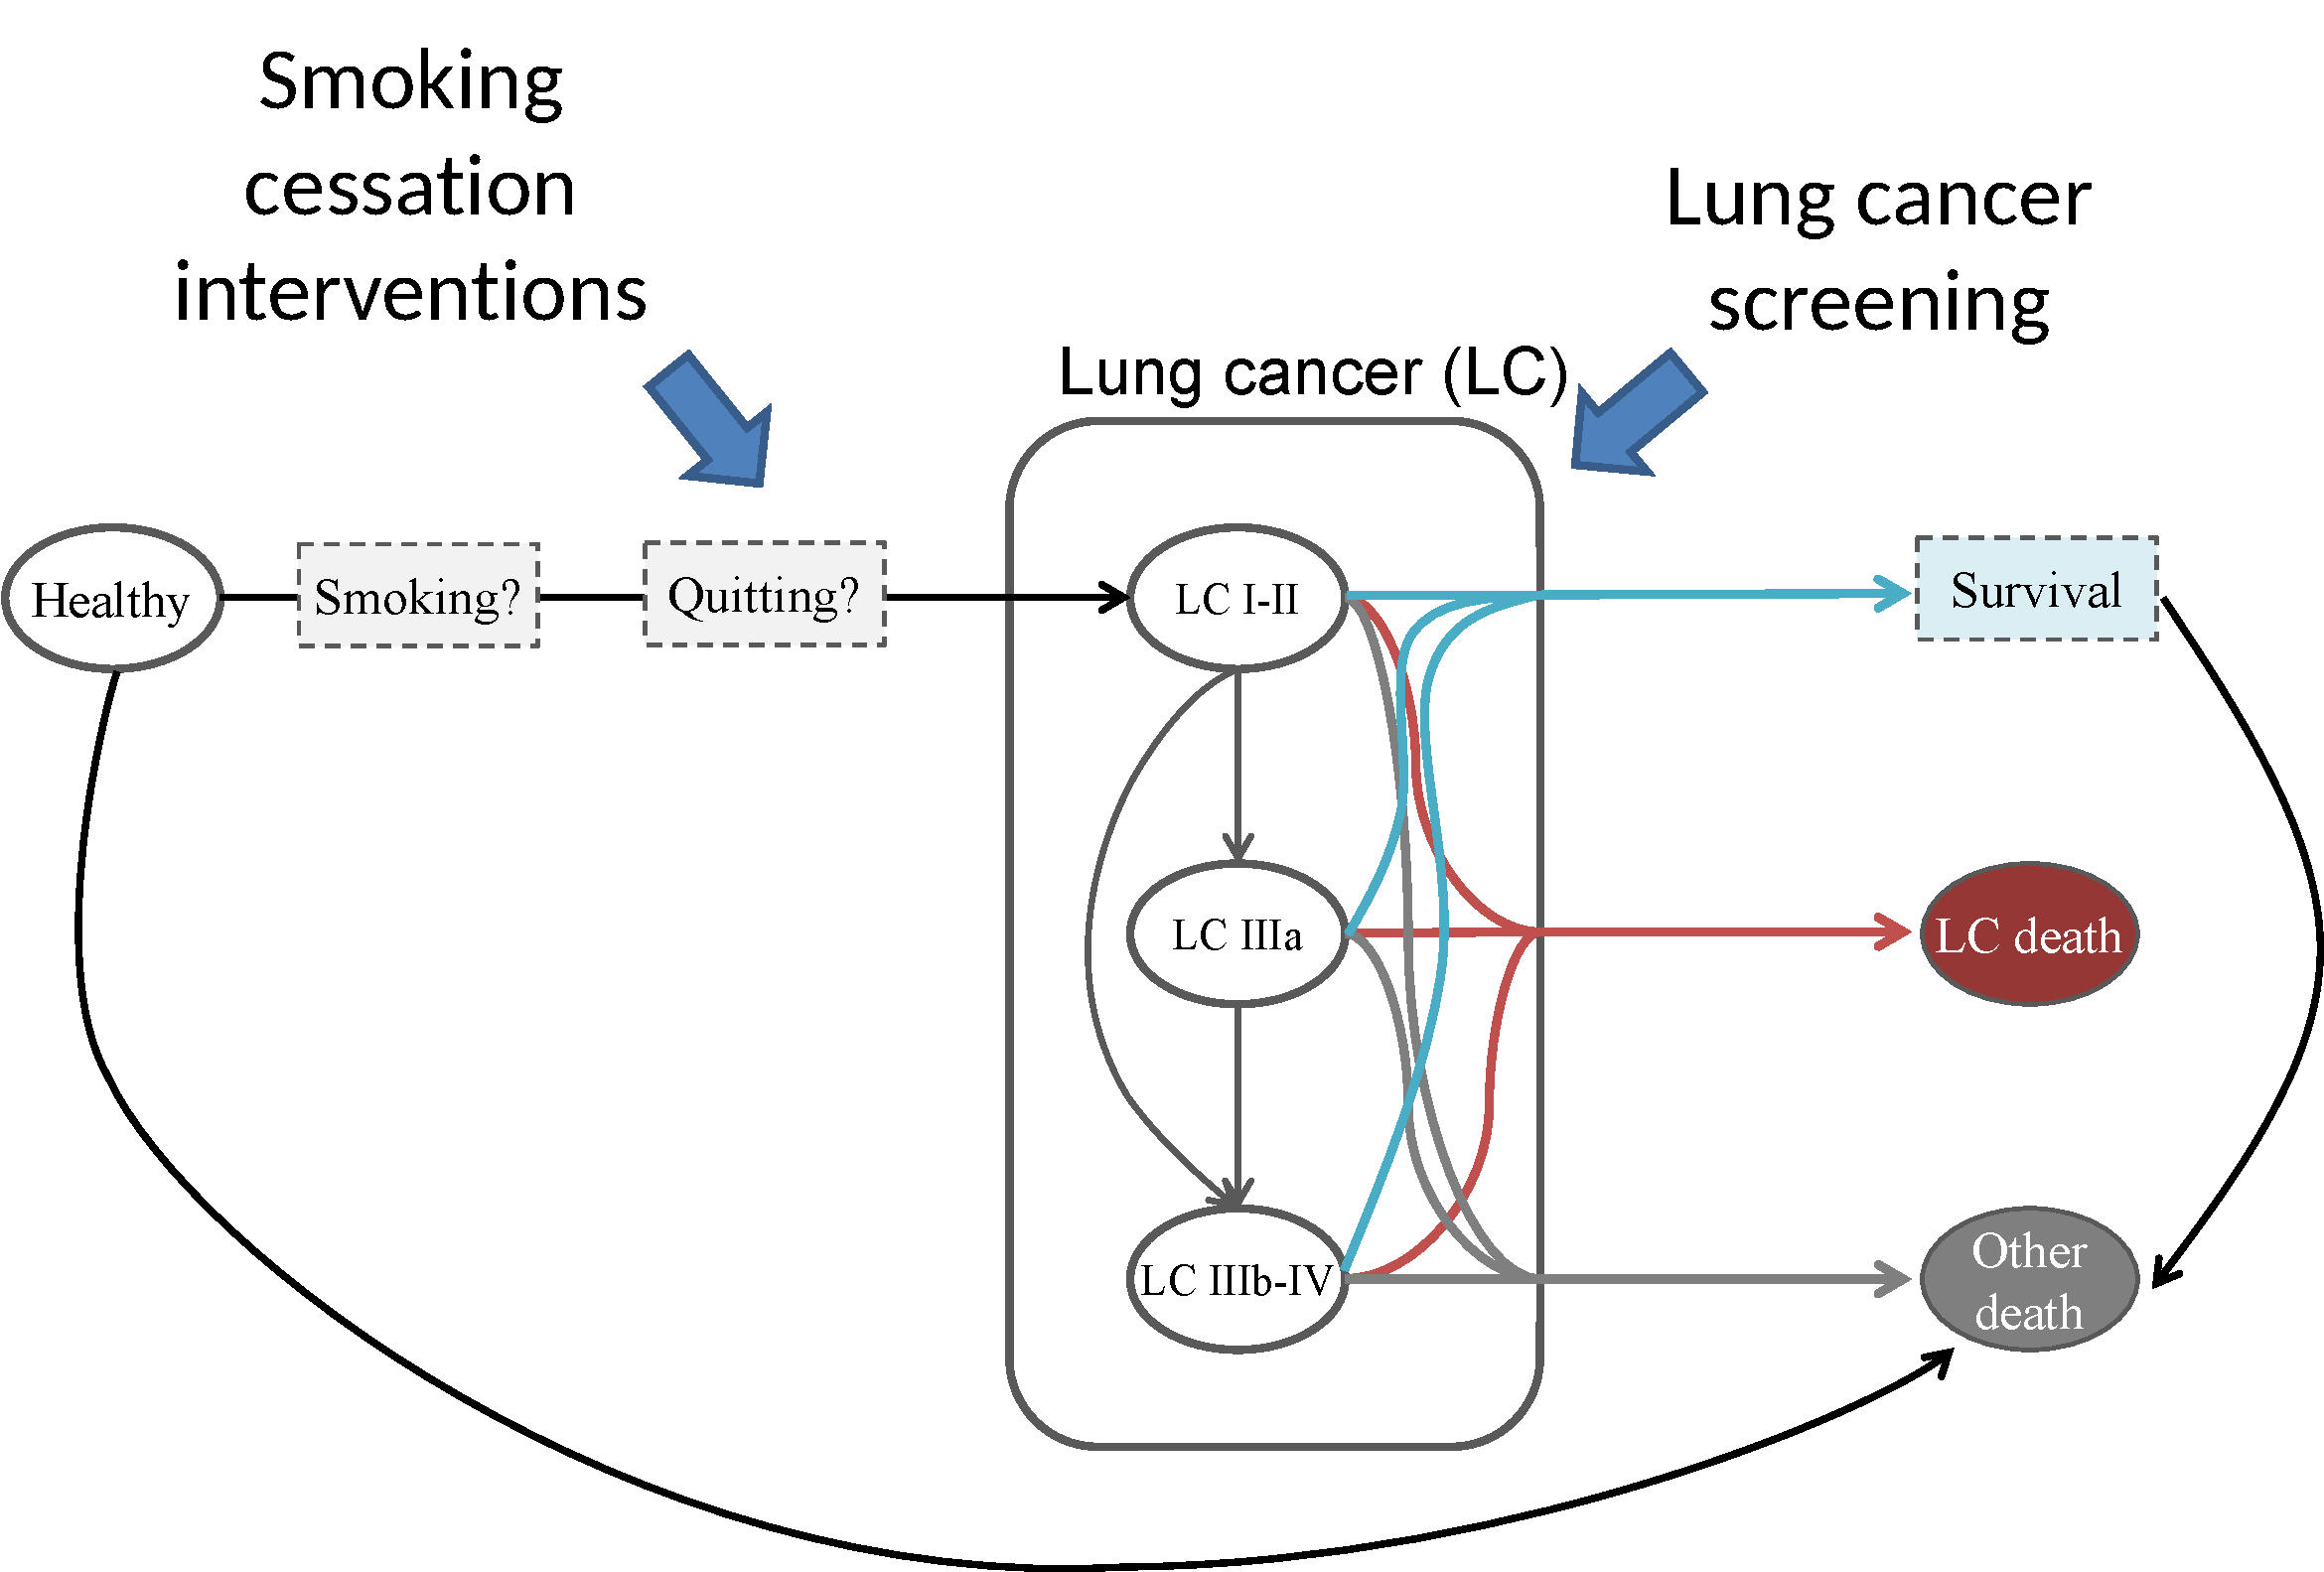
\includegraphics[width=80mm]{figs/lungmodel.pdf}		
		\caption{Lung cancer markov model state diagram}	
		\label{fig:lung_model}	
	\end{figure}
	
	By comparing the incremental cost-effectiveness ratio (ICER) of two strategies (equation \ref{eq:icer}), we can determine the additional expenditure required to increase life expectancy by one year if the second strategy is adopted\cite{drummond}. This ICER can then be compared to a willingness-to-pay threshold determined by the geographical region, with strategies with ICERs falling below the threshold considered cost-effective.
	
	\begin{equation}
		\label{eq:icer}
		\textnormal{ICER}=\frac{\Delta \textrm{Cost}}{\Delta \textrm{Effectiveness}} = \frac{C_2-C_1}{E_2-E_1} \quad [\euro{}/\textrm{QALY}]
	\end{equation}
	
	In order to execute the simulations, input parameters are required to describe the disease process, such as probabilities, hazard ratios, or disease burden rates extracted from scientific literature. Due to the inherent uncertainty of these values, it is often necessary to calibrate the model before proceeding with the analysis. Calibration consists in adjusting the input parameters until the resulting output approximates a target value identified in the scientific literature, such as disease incidence, prevalence, or mortality. This optimization process can be especially taxing for complex models, and may necessitate the use of advanced techniques to efficiently explore the solution space.
	
	Moreover, calibrations can be highly dimensional optimization problems with many arbitrary constraints between parameters, dictated by the specific medical domain. In this work, we explore the challenges associated with calibrating simulation models and propose methods to overcome them. Our research provides valuable insight into novel ways to calibrate these simulation models more efficiently using Bayesian Optimization. We also investigate the circumstances under which it outperforms common methods used in the field.	
	
	
	\section{Background}
	
	% Nice description out of ChatGPT. Maybe we could include citations and adapt a bit? 
	% Cite: Garnett, R. (2023). Bayesian optimization. Cambridge University Press.
	\subsection{Bayesian Optimization}
	
	Bayesian optimization is a powerful technique for optimizing expensive, black-box functions that are difficult or time-consuming to evaluate. The basic idea is to build a probabilistic model of the function based on the observations made so far, and then use this model to guide the selection of new points to evaluate. The method is particularly useful when the objective function is complex and has multiple input variables.
	
	At the heart of Bayesian optimization is a probabilistic model, typically a Gaussian process, that captures our beliefs about the unknown function we are trying to optimize. The GP provides a distribution over functions that is consistent with the observed data, and allows us to reason about the uncertainty associated with our predictions. We start by selecting a few initial points to evaluate, and use these to fit the GP model. We then iteratively select new points to evaluate based on a trade-off between exploration (trying to find regions of the input space with high uncertainty) and exploitation (trying to find regions with high predicted performance).
	
	The key advantage of Bayesian optimization is that it can find the global optimum of the function with relatively few evaluations, even in high-dimensional spaces. This is because the method actively seeks out the most promising areas of the input space to evaluate next, rather than simply evaluating points at random. The downside is that the method can be computationally expensive, especially for functions with a large number of input variables or when the GP model is complex.
	
	Bayesian optimization has been successfully applied to a wide range of optimization problems in machine learning, including hyperparameter tuning, experimental design, and automatic algorithm configuration. In these applications, the objective function is often a performance metric that is expensive to evaluate, such as the validation error of a machine learning model. Bayesian optimization can help to quickly identify good values of the hyperparameters or experimental conditions, without having to exhaustively search the entire parameter space.
	
	\subsection{Gaussian Processes}
	Gaussian Processes (GPs) are non-parametric regression models that represent each observation as a random variable drawn from a Gaussian distribution $f(x) \sim \mathcal{N}(\mu(x), k(x,x))$\cite{gaussian-processes}. The mean function $\mu(x)$ and the covariance function $k(x,x')$ define the expected value of the Gaussian Process and the degree of dissimilarity between different inputs, respectively. For an assumed noise level in the data $\sigma^2$, an initial prior $\mu_0(X)$ (often $\mu_0(X)=0$), a given observation set $X=\{\vec{x_1}, ..., \vec{x_D}\}$ with labels $\vec{y}$ and a Gram matrix $K$ built from $X$ and a set of unknown observations $X_*$, a Gaussian Process $f_*$ has an analytic form for the predictive posterior distribution (equation \ref{eq:predictive_posterior}).% and the marginal loglikelihood function (equation \ref{eq:loglikelihood}).
	%Bayesian Optimization (BO) is a sequential model-based technique to optimize a given target function. This approach encapsulates our knowledge about the target function in a probabilistic model and uses it to guide the optimization process. This surrogate model starts with a prior distribution, which reflects our initial assumptions about the function, and is updated as new data is gathered. The acquisition function, which measures the promise of a new observation and directs how the search space should be explored, is maximized to identify the next point to evaluate. This process is repeated until a satisfactory solution is found, or a termination criterion is met.
	
	%One popular choice for surrogate models are Gaussian Processes. These non-parametric regression models represent each observation as a random variable drawn from a Gaussian distribution $f(x) \sim \mathcal{N}(\mu(x), k(x,x))$. The mean function $\mu(x)$ and the covariance function $k(x,x')$ define the expected value of the Gaussian Process and the degree of dissimilarity between different inputs, respectively. For an assumed noise level in the data $\sigma^2$, an initial prior $\mu_0(X)$ (often $\mu_0(X)=0$), a given observation set $X=\{\vec{x_1}, ..., \vec{x_D}\}$ with labels $\vec{y}$ and a Gram matrix $K$ built from $X$ and a set of unknown observations $X_*$, a Gaussian Process $f_*$ has an analytic form for the predictive posterior distribution (equation \ref{eq:predictive_posterior}) and the marginal loglikelihood function (equation \ref{eq:loglikelihood}).
	
	\begin{equation} \label{eq:predictive_posterior}
		\begin{aligned}
			f_*|X,\vec{y},X_* & \sim \mathcal{N}(\mu(X_*), \Sigma(X_*)) \\
			\mu(X_*) & = \mu_0(X_*) + K(X_*,X)(K(X,X) + \sigma^2 I)^{-1}(\vec{y} - \mu_0(X_*)) \\
			\Sigma(X_*) & = K(X_*,X_*) + \sigma^2 I - K(X_*,X)(K(X,X) + \sigma^2 I)^{-1} K(X,X_*)
		\end{aligned}
	\end{equation}	

	%\begin{equation} \label{eq:loglikelihood}
	%	\begin{aligned}
	%		\log{p(\vec{y}|X)} &= -\frac{1}{2}\vec{y}^T (K(X,X) + \sigma^2 I)^{-1}\vec{y} - \frac{1}{2}\log{|K(X,X) + \sigma^2 I|} - \frac{n}{2}\log{2\pi}
	%	\end{aligned}
	%\end{equation}	

	%\begin{equation}
	%	\begin{aligned}
	%		K(X,X') &= K\left(\begin{bmatrix} \vec{x_1} \\ \vdots \\ \vec{x_m} \end{bmatrix}, \begin{bmatrix} \vec{x'_1} \\ \vdots \\ \vec{x'_n} \end{bmatrix}\right) = \begin{bmatrix} 
	%			k(x_1,x'_1) & \dots  & k(x_1,x'_n)\\
	%			\vdots & \ddots & \vdots\\
	%			k(x_m,x'_1) & \dots  & k(x_m,x'_n)
	%		\end{bmatrix}
	%	\end{aligned}
	%\end{equation}
	
	The covariance function or kernel is the mechanism to give a Gaussian Process its expressive power, and its choice will heavily depend on the kind of function we aim to model\cite{kernel-composition}. The squared exponential (SE) kernel $k(x,x') = \sigma^2 e^{-\frac{||x-x'||^2}{2l^2}}$ is a popular choice, despite significant drawbacks such as its locality and sensitivity to the curse of dimensionality\cite{curse-dimensionality}.
	In general, modeling complex high dimensional functions using a single kernel can be computationally expensive using local kernels, making this a first class research problem (e.g. \cite{gp-high-dim}\cite{gp-high-dim2}).
	%As a result, the SE kernel can be an inefficient option in many high-dimensional Bayesian Optimization problems.
	%Many techniques are under active research to address high-dimensional problems with Gaussian Processes 
	Additive kernel decomposition\cite{gp-additive} addresses this problem by breaking down the kernel into a sum of simpler kernels, each of which captures a different aspect of the relationship between the input variables. This approach can capture both local and global interactions between the input variables. Additionally, additive kernel decomposition can improve the interpretability of the model, as each kernel term can be associated with a specific interaction term. This can help users understand which orders of interaction are important for the current optimization problem. 
	%One of these techniques is additive kernel decomposition\cite{gp-additive}.
	%The full additive kernel is shown in equation \ref{eq:additive1} as the weighted sum of the additive kernels of all order interactions (equation \ref{eq:additive2}), when a SE kernel is used as the base kernel (equation \ref{eq:additive3}).
	
	
	%\begin{align}
	%	k_{add}(x,x') &= \sum_{i=1}^D{\sigma_i^2 k_{add_i}(x_i,x_i')} \label{eq:additive1}\\
	%	k_{add_j}(x,x') &= \sum_{1\leq i_1 < i_2 < \ldots < i_j\leq D} \left[\prod_{d=1}^{j} k_{i_d}(x_{i_d},x_{i_d}') \right] \label{eq:additive2}\\
	%	k_i(x,x') &= e^{\frac{(x_i-x_i')^2}{2l_i^2}} \label{eq:additive3}
	%\end{align}
	
	
	Additive kernels suffer from the non-identifiability problem: the kernel hyperparameters are not uniquely identifiable from the observed data, which can lead to challenges in model selection and interpretation.
	To ensure a unique decomposition, Lu et al\cite{gp-additive-orthogonal} proposed an extension of additive kernels by including an extra constant kernel $\tilde{k}_{add_0}(x,x')$ with an additional variance hyperparameter $\sigma_0^2$ and an orthogonality constraint to generate Orthogonal Additive Kernels (OAK)\cite{gp-additive-orthogonal}. Assuming a normal input distribution $x_i \sim \mathcal{N}(\mu_i, \delta_i^2)$, the following constrained base kernel is derived:
	
	\begin{equation} \label{eq:additive-orthogonal}
		\begin{aligned}
			k_{add_{OAK}}(x,x') &= \sum_{i=0}^D{\sigma_i^2  \tilde{k}_{add_i}(x_i,x_i')} \\
			%\tilde{k}_{add_0}(x,x') &= 1\\
			\tilde{k}_{add_j}(x,x') &= \sum_{1\leq i_1 < i_2 < \ldots < i_j\leq D} \left[\prod_{d=1}^{j} \tilde{k}_{i_d}(x_{i_d},x_{i_d}') \right]\\		
			\tilde{k}_i(x,x') &= e^{\frac{(x_i-x_i')^2}{2l_i^2}} - \frac{l_i\sqrt{l_i^2 + 2\delta_i^2}}{l_i^2 + \delta_i^2} e^{-\frac{(x_i-\mu_i)^2 + (x_i'-\mu_i)^2}{2(l_i^2 + \delta_i^2)}}
		\end{aligned}
	\end{equation}
	
	One important advantage of these additive kernels is that we can interpret the $\sigma_i^2$ as the contribution of each individual order to the total kernel. Since many problems often rely on a few low-order interactions, we can truncate the higher orders and limit the computational cost while retaining most of the information present in the full decomposition. To achieve this, OAK kernels can be useful in accurately identifying each contribution and providing an accurate representation on the actual composition on the function.
	
	\section{Methodology}
	In this section we will describe the simulation model and the optimization methods we will use to calibrate it. These include the Bayesian method and the rest of techniques that will be compared.
	
	\subsection{Description of the Simulation Model}
	\label{sec:simulation-model}
	We use a lung cancer model presented in a published cost-effectiveness analysis\cite{lung-model} as a fast benchmark for Bayesian Optimization on simulation models. This Markov-based microsimulation model simulates a cohort's progression through seven different health states over time. The transition probabilities used in the model were age-specific, with distinct values for each 5-year age group (35-39, 40-44, ..., 75-79). The state diagram for this model is pictured in figure \ref{fig:lung_model}.
	
	To simplify the calibration tests, certain simulation details were ignored in the original model, such as gender differentiation, smoking prevalence, and quitting probabilities for smokers. Additionally, the survival health state was removed, resulting in only six states being considered and 6x6 transition matrices being used. Certain inherent constraints, such as ensuring that the sum of the probabilities in each row equals one or that certain probabilities are zero, were imposed on the matrices. This allowed the number of parameters to be optimized per age group to be reduced from 36 to 11. Among these nine age groups, each with its own set of 11 parameters, only the first few of these were calibrated in this study. As a result, the problem was simplified to the calibration of 11 parameters, rather than the original $11\cdot 9=99$ parameters associated with the full simulation. Furthermore, this model was designed to be computationally inexpensive, taking less than 10ms to simulate. By introducing arbitrary delays in the model we can observe the relationship between calibration times and model simulation times for different optimization methods.
		
	Another important component for these simulation models are parameter constraints. One common, non-trivial constraint present in similar models are age-dependent parameters following a particular trend. For example, in this lung cancer model we will consider an increasing trend for the probability of developing cancer at age group $i$: $p_c^{(i)}$. This gives us the following global constraint:
	
	\begin{equation} \label{eq:constraint}
		\begin{aligned}
			p_c^{(1)} < p_c^{(2)} < \dots < p_c^{(9)}	
		\end{aligned}
	\end{equation}
		
	The calibration target for the model was defined as the weighted sum of the euclidean distances between the observed and expected outputs of interest, namely lung cancer incidence (45\%), lung cancer mortality (45\%) and mortality from other causes (10\%), computed for each age group.
	
	
	\subsection{Optimization Methods}
	In cost-effectiveness modeling, it is common to have an initial estimate of a good solution based on approximate values found in the scientific literature. For all optimization experiments conducted, a solution space of plus or minus $\pm 50\%$ was considered for each input variable, centered around this initial value.
	
	First, we used different optimization methods to illustrate the performance differences between regular Bayesian Optimization and classical methods. For this purpose we used python implementations of commonly used methods: a hill-climbing technique (Nelder-Mead\footnote{\url{https://docs.scipy.org/doc/scipy/reference/optimize.minimize-neldermead.html}}\cite{nelder-mead}), metaheuristics (Simulated Annealing (SA)\footnote{\url{https://docs.scipy.org/doc/scipy/reference/generated/scipy.optimize.dual_annealing.html}}\cite{simulated-annealing} and Particle Swarm Optimization\footnote{\url{https://pyswarms.readthedocs.io/en/latest/}}\cite{pso}), and Bayesian Optimization with Gaussian Processes using Squared Exponential kernels (BO-SE)\footnote{\url{https://secondmind-labs.github.io/trieste/1.1.2/index.html}}. The default hyperparameter values were used for these methods, except for Particle Swarm Optimization, where the number of particles was set to 1,000 times the number of age groups calibrated.
	
	We also developed a new BO implementation with Gaussian Processes using the R programming language. This implementation was used as a rapid prototyping environment to evaluate different enhancements to the optimization process for our specific domain, without being concerned by execution time at this stage. This implementation uses the Expected Improvement acquisition function (equation \ref{eq:expected-improvement}, where $x^+$ represents the best optimum found so far), with Particle Swarm Optimization to search for its maximum. Finally, both the SE and the OAK kernels (BO-SE and BO-OAK) were implemented. Runtime optimizations such as GPU use are beyond the scope of this work.
	
	\begin{equation} \label{eq:expected-improvement}
		\begin{aligned}
			\text{EI}(x) &= \mathbb{E}[\max(f(x)-f(x^+), 0)]
		\end{aligned}
	\end{equation}

	Before starting the BO procedure we learn the lengthscales $l_1, ..., l_D$ and the variances $\sigma_0^1, \sigma_1^2, ..., \sigma_n^2$ of the OAK kernel in a two stage process. In the first stage, we maximize the marginal likelihood for each lengthscale separately. In the second stage, we maximize the marginal likelihood for the whole set of variances. This approach allows us to break down a complex task for high-dimensional problems into low-dimensional, manageable problems. This is particularly important when working with larger models.
	
	\subsection{Constrained optimization methods}
	\label{sec:constrained-optimization}
	 In the methodology described so far we have not considered the parameter constraints such as (\ref{eq:constraint}). A naive, method-agnostic constraint handling technique could consist in heavily penalizing the error function when the parameters don't satisfy (\ref{eq:constraint}). For BO, one way to implement constraint handling is by using the constrained Expected Improvement (cEI) acquisition function\cite{bo-constraints1}, which balances the fitness of the observations with its feasibility.
	
	Gardner's method can be extended to several constraints and used in this problem by decomposing (\ref{eq:constraint}) in a series of simple constraints:
		
	\begin{equation} \label{eq:constraint-simple}
		\begin{aligned}
			p_c^{(1)} &- p_c^{(2)} < 0 \\
			p_c^{(2)} &- p_c^{(3)} < 0 \\
			&\dots \\
			p_c^{(8)} &- p_c^{(9)} < 0 \\
		\end{aligned}
	\end{equation}

 But in doing so the covariance between restrictions should be considered or independence between constraints should be assumed. Even though often this dependence assumption can be safely disregarded\cite{bo-constraint-dependence}, in some cases it might be relevant to consider in order to efficiently explore the solution space. 	
 	
 	
 	\subsection{Stepwise calibration}
 	Calibrating under constraints can be as straightforward as solving a singular constrained optimization task using the methods described in section \ref{sec:constrained-optimization}. Depending on the kind of constraints and the dimensionality of the problem that might be unfeasible computationally and other approaches can be more suited to the structure of our simulation models.
 	
 	We will use a greedy method to calibrate efficiently that we will call stepwise calibration. As we mentioned in section \ref{sec:simulation-model}, these simulation models follow a sequential structure that is dependent on time: the output of the simulation for one age group depends only on the relevant parameters for that age group and those preceding them, not on those of later age groups.
 	
 	Let $f(\bm{p})$ be the output or final state of the full simulation model given parameters $\bm{p} = \{p_1, p_2, ..., p_n\}$. We can make a partition $p^{(i)}$ of these parameters, according to the age group $i$ they influence so that $\bm{p} = p^{(1)} \cup p^{(2)} \cup ... \cup p^{(k)}$. With this partition, and the partial states for each age group ($s_i$), we can reformulate the final state of the model $f(\bm{p}) = s_k$ as:
 	
 	\begin{equation} \label{eq:stepwise-function}
 		\begin{aligned}
 			s_1 &= f_1(p^{(1)}) \\
 			s_2 &= f_2(p^{(2)} \mid s_1) \\
 			s_3 &= f_3(p^{(3)} \mid s_2) \\
 			&\dots \\
 			f(\bm{p}) = s_k &= f_k(p^{(k)} \mid s_{k-1}) \\ %= f_1(p^{(1)}) \circ f_2(p^{(2)}) \circ \dots \circ f_k(p^{(k)})\\
 		\end{aligned}
 	\end{equation}	
 	
 	This decomposition allows a greedy approach where we can break down the calibration of the full model $f(\bm{p})$ into $k$ tasks by iteratively calibrating each age group conditionally to the previously calibrated parameter groups, as described in algorithm \ref{alg:stepwise}.
 	
 	\begin{algorithm}[h!]
 		\caption{Stepwise calibration with $k$ age groups}\label{alg:stepwise}
 		\begin{algorithmic}
 			\State $\mathrm{target} \gets [t_1, \dots, t_k]$
 			\For{$i$ from 1 to $k$} \\
 			\State $p_*^{(i)} \gets \underset{p^{(i)}}{\mathrm{argmin}}\, \norm{f_i\left(p^{(i)} \mid p_*^{(1)}, \dots, p_*^{(i-1)}\right) -  t_i}$
 			\EndFor
 			\State \Return $[p_*^{(1)}, \dots, p_*^{(k)}]$
 		\end{algorithmic}
 	\end{algorithm}
 	
 	As expected from a greedy method, the optimum for each step does not guarantee being part of a global optimum, and each solution found by these subcalibrations might lead to suboptimal solutions in subsequent subcalibrations. On the other hand, This method lowers the dimensionality of the full calibration into $k$ smaller optimization problems, reducing the overall computational effort.
 	
 	An important advantage of this method is that it can simplify constraints with similar structure to equation \ref{eq:constraint-simple}. Stepwise calibration transforms equations \ref{eq:constraint-simple} in single constraints conditional to the optimal value of the parameter found in the previous optimization step:
 	
 	\begin{equation} \label{eq:stepwise-function}
 		\begin{aligned}
 			p_c^{(i)} - p_{c*}^{(i-1)} < 0
 		\end{aligned}
 	\end{equation}	
 
 	where $p_c^{(i)} \in p^{(i)}$.
 	
 	Finally, it should be noted that stepwise calibration is a technique that can be used with any optimization method, in both constrained and unconstrained settings.
 
	\section{Results}
	
	\subsection{Unconstrained calibration}
	\label{sec:results-unconstrained}
	Our interest in these experiments are about the comparative performance of BO versus the rest of methods in the calibration of simulation models, without considering the constraints stated in (\ref{eq:constraint}). We can see the relationship between simulation time and calibration time for each method in figure \ref{fig:sim_times}. For very fast models the inference overhead of BO dominates and other methods are able to calibrate faster by simulating the model many times. However, as the simulation time increases, the Bayesian method efficient approach in number of function evaluations results in faster calibration times. Specifically, for a model with 11 parameters and simulation times greater than 0.25s we observed the Bayesian approach outperform the alternative methods. We will call this threshold the critical simulation time.
	
	In contrast, as the dimensionality of our problem grows, the bayesian method overhead increased significantly, as shown in the y-intercept of figure \ref{fig:sim_times}. The calibration times for the other methods also increased but, overall, the critical simulation time increases exponentially with the number of parameters, from 0.2 seconds to 0.35, 0.95 and 3.25 seconds. The bottom left plot in figure \ref{fig:sim_times} projects that for all 99 parameters BO-SE would be the fastest technique when each simulation takes approximately 5 minutes of computation.
	
	\begin{figure}[h!]
		\centering	
		\includegraphics[width=\textwidth]{figs/crit\_times\_log.pdf}		
		\caption{Total calibration time in log scale against model simulation time required to attain similar levels of error. The bottom left figure shows the exponential trend (in log scale) in the critical simulation time as a function of the number of parameters. The bottom right figure is a zoomed-in plot of the same figure removing the log scale.}
		\label{fig:sim_times}	
	\end{figure}
	
	In any case, the focus of our research in this work is the number of evaluations, where we see a sharp drop in error when using BO to achieve a similar level of accuracy compared to other methods, as shown in figure \ref{fig:method_comparison}. Although each iteration requires a significant amount of time due to the bayesian inference step, this overhead will become less relevant as the size of the model increases.
	
	\begin{figure}[h!]
		\centering	
		\includegraphics[width=\textwidth]{figs/methods\_n1.pdf}		
		\caption{Time series of the lung cancer model calibration error (using 1 age group). The error is plotted against the number of evaluations by method.}
		\label{fig:method_comparison}	
	\end{figure}
	
	While exploring the results of BO-OAK we found that one of the variables had very significant explanatory power by itself, which could produce misleading results in the comparison. To address this issue, we introduced a third univariate SE kernel that considers only this variable. Figure \ref{fig:results_oak} shows the average progression of the error during the optimization process for the three kernels and their interquartile range for a sample of 30 random executions. The univariate SE kernel shows a lower average error and lower spread than the full SE kernel, due to the reduction in dimensionality of the problem that allows for an easier exploration of the solution space, with barely any information loss. However, the OAK kernel under a normality assumption for the inputs is able to efficiently search the full 11-dimensional space to reach even better average results than the univariate SE kernel, while reducing the dispersion as the optimization progresses.
	
	\begin{figure}[h!]
		\centering	
		\includegraphics[width=\textwidth]{figs/results\_q.pdf}		
		\caption{Time series of the median BO error with its interquartile range as the shaded area. We used three different kernels: the SE kernel (blue), the univariate SE kernel using only the most significant variable (green) and the OAK kernel under a normality assumption for the inputs (red).}
		\label{fig:results_oak}	
	\end{figure}

	\subsection{Constrained calibration}
	When considering constraints such as equation \ref{eq:constraint} it was found to be unfeasible to calculate in a reasonable amount of time. Even considering a four age group model with the first three constraints ($p_c^{(1)} < p_c^{(2)}$, $p_c^{(2)} < p_c^{(3)}$, $p_c^{(3)} < p_c^{(4)}$), BO-OAK had trouble finding valid solutions in a reasonable amount of time, taking many hours of computation. Other adhoc techniques could be used to improve the search with this particular constraint but a more general approach was preferred.
	
	Using stepwise calibration lowered the computational cost dramatically for BO, allowing us to perform the full calibration for all nine age groups in a feasible time. We transformed an optimization task of 99 parameters to 9 optimization tasks of 11 parameters each, reducing the exponential impact of the number of parameters. Furthermore, the critical simulation times are drastically reduced as well, as we can see in figure \ref{fig:crit-times-constrained}. Note that BO-SE using a conventional calibration had a projected critical simulation time around 300s for the full model (see figure \ref{fig:sim_times}), where in the stepwise calibration the critical time of the same method is reduced to 0.24s. Focusing on which is the fastest calibration method given a simulation time, we can differentiate three regions in table \ref{tab:crit-times-constrained}.
		
	\begin{figure}[h!]
		\centering	
		\includegraphics[width=\textwidth]{figs/crit\_times\_constrained.pdf}		
		\caption{Total stepwise calibration time in log scale against the full model simulation time required to attain similar levels of error. Two different x-axis scales are presented to properly show the two relevant points of interception for the BO methods.}
		\label{fig:crit-times-constrained}	
	\end{figure}

	\begin{table}[h!]
		\begin{tabular}{lll}
			\textbf{\begin{tabular}[c]{@{}c@{}}Simulation time\end{tabular}} & \textbf{\begin{tabular}[c]{@{}c@{}}Fastest stepwise\\ calibration method\end{tabular}}  \\
			$< 0.24$s  & Nelder-Mead \\
			$0.24$s - $120$s & BO-SE  \\
			$> 120$s & BO-OAK
		\end{tabular}
		\caption{Critical simulation times for simulation model with nine age groups as seen in figure \ref{fig:crit-times-constrained}.}
		\label{tab:crit-times-constrained}	
	\end{table}

	Stepwise calibration also manages to find solutions for our simulation model with comparable error than those found by regular calibration or even lower. In particular we can compare the error for the first age group of figure \ref{fig:stepwise-error} (0.13) with the error obtained in figure \ref{fig:method_comparison} (0.65). In the BO-OAK case we see that the error is significantly reduced in the first and last few age groups while increased in the middle ones, managing to find a better overall solution.
	
	Notice that the sharp increase in error in age group 7 is shared among all methods. The cause of this effect is due to the nature of the simulation and how the target has been chosen. It is therefore a limitation of the simulation model and not an optimization artifact.
	
	\begin{figure}[h!]
		\centering	
		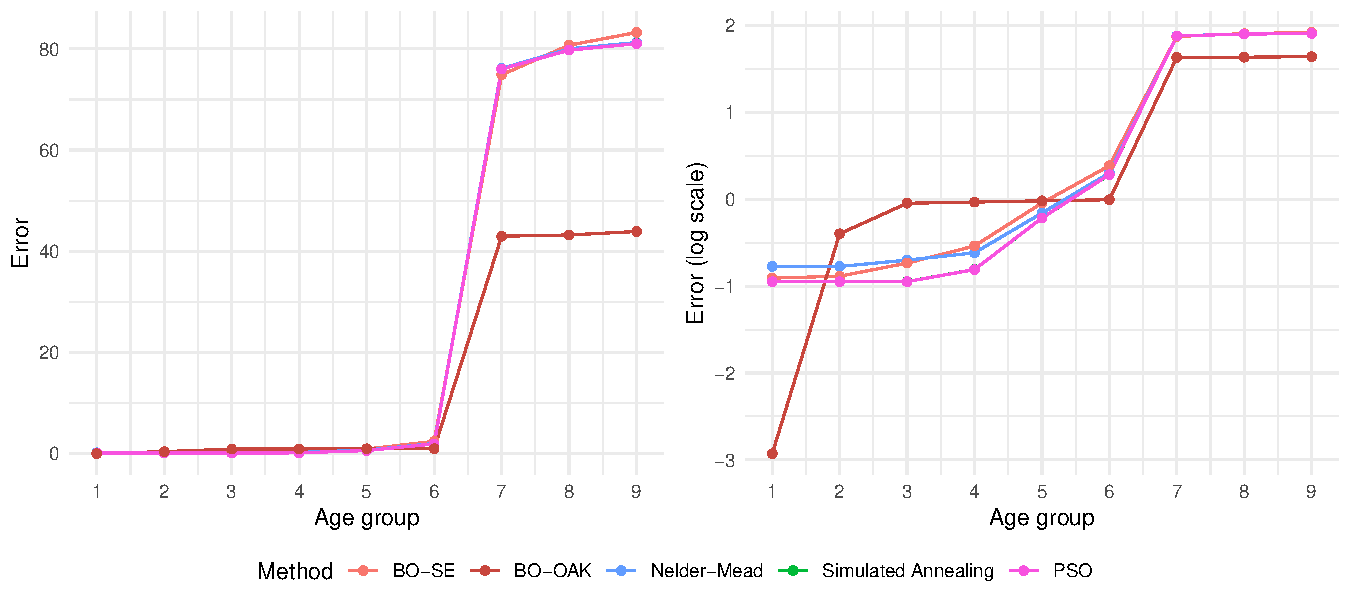
\includegraphics[width=\textwidth]{figs/stepwise_error.pdf}		
		\caption{Stepwise calibration error for each age group in linear scale (left) and log scale (right).}
		\label{fig:stepwise-error}	
	\end{figure}

	\section{Discussion}
	BO is currently considered a state-of-the-art optimization method in various domains that involve costly functions to evaluate. When the computational cost of the objective function is large enough, Bayesian Optimization might be the natural choice. But when the function is not as expensive, there are two other critical points in each BO iteration that must be taken into account: the surrogate model regression and the acquisition function optimization.
	
	The optimization of the acquisition function is the initial bottleneck, where the number of observations is still small enough so that the surrogate model regression is not yet a problem. As the search space remains constant, this acquisition optimization doesn't become much more expensive as more data is observed. We used Particle Swarm Optimization as an easy way to take advantage of parallelism in this area, but other approaches mentioned in the next section are being considered as well\cite{acquisition-functions}.
	
	Regarding the surrogate model regression, SE kernels suffer greatly from the curse of dimensionality. In high-dimensional problems, the number of observations to explore the solution space quickly increases. This renders the regression unfeasible when trying to invert large Gram matrices to calculate the posterior predictive distribution. To address this issue, OAK kernels can reduce the number of necessary observations, mitigate the effects of an expanding Gram matrix and enhance the efficiency of the search. The observed scaling issues in figure \ref{fig:sim_times}, resulting from increasing dimensionality, justify the need for high-dimensional improvements such as OAK kernels. Nevertheless, our experiments showed that the asymptotic behaviour of Bayesian Optimization persisted, making it the optimal choice for sufficiently large models.
	
	Another way to deal with high-dimensionality for simulation models in a more effective way is to use stepwise calibration. Using this technique allows us to calibrate models that are prohibitive using other methods by reducing a high number of parameters to a sequence of calibrations with fewer parameters. Stepwise calibration is reasonable to use when the target function has a inherent sequential block structure, but as many greedy algorithms even if each step makes an optimal choice it does not guarantee that the global solution built from those is optimal as well. We are confident in the suitability of this technique for our simulation models for two reasons: in first place the solutions found in our results have a similar error to those found using conventional calibration, or even lower in the case of BO-OAK. Secondly, we have seen that the tuned OAK hyperparameters assign a negligible weight to the orders of interaction greater than one, so we can infer that the interaction between parameters is not too complex and the greedy approach should be a reasonable approximation for many problems where only the first orders of interaction are important\cite{gp-additive}.
	
	These two techniques, BO-OAK and stepwise calibration, can be combined with impressive results, finding better solutions than the rest of methods in a shorter time as long as the simulation model is moderately time-consuming ($\sim 2$ minutes). These results hold in spite of a BO-OAK implementation that can be highly improved during the kernel numerical computation. A properly optimized implementation could speed up the calibration process and reduce the critical time even further.
		
	Lu et al\cite{gp-additive-orthogonal} mention that an interesting direction of work would be to extend OAK kernels to Bayesian Optimization leveraging the inferred low-order representation. In our tests we show that, even with a straightforward application of OAK kernels on this simple example, a slight improvement over the SE kernel is noticeable. This improvement is expected to be more meaningful for complex models, where more structure can be leveraged. It is interesting to note that these results hold even though some assumptions of the model were not met. Specifically, hyperparameter tuning was performed with a dataset sampled from a uniform input distribution, while the constrained kernels were calculated assuming normality in the input. Even if these distributions were consistent, we still would have the problem of determining the input distribution for the actual optimization process, which would be neither normal nor uniform.
	
	%gp max likelihood ill-posed -> impose gaussian noise
	
	\section{Future Work and Conclusions}
	One particular aspect that we did not incorporate into this article is constraint handling. Simulation models can be highly constrained problems, and these constraints are another expression of the structure of the solution space. We have been able to manage arbitrary constraints successfully using additional surrogate models and a new Constrained Expected Improvement acquisition function, as introduced by Gardnet et al\cite{gp-constraints}.
	
	We also mentioned in the discussion the convenience of exploiting the parallelization potential of the different areas of the optimization process. For that purpose we use the Particle Swarm method for the optimization of the acquisition function, but other more sophisticated venues for parallelization include batched optimization\cite{gp-batch}, parallel acquisition functions\cite{gp-parallel-acq-func} or GPU approaches\cite{gp-gpu} among others.
	%Removed \cite{gp-batch2}
	
	Our research group recognizes the importance of efficiently calibrating increasingly complex models, injecting relevant domain knowledge in the process. In this work we have shown that using OAK kernels in a BO setting allows faster calibration times under very common circumstances in the health economics field. This is the beginning of several enhancements that are being implemented to have the tools to work with more challenging models in the future.
	
	\section{Acknowledgement}
	This work was supported by a grant from the Instituto de Salud Carlos III-ISCIII (Spanish Government) co-funded by European Regional Development Fund, a way to build Europe (CIBERESP CB06/02/0073, PI19/01118), also with the support of the Secretariat for Universities and Research of the Department of Business and Knowledge of the Government of Catalonia. Grants to support the activities of research groups (SGR 2017–2021). Grant number 2021SGR1029. We thank the CERCA Programme and Generalitat de Catalunya for institutional support.
	
	
	
	\begin{thebibliography}{99}
		
		\bibitem{drummond}
		Drummond MF, Sculpher MJ, Claxton K, Stoddart GL, Torrance GW, Drummond MF, et al. Methods for the Economic Evaluation of Health Care Programmes. Fourth Edition, Fourth Edition. Oxford, New York: Oxford University Press; 2015. 464 p. doi: 10.1002/(SICI)1099-176X(199903)2:1<43::AID-MHP36>3.0.CO;2-7
				
		\bibitem{levin}
		Levin HM. Cost-Effectiveness Analysis: Methods and Applications. 2nd edition. Thousand Oaks, Calif: SAGE Publications, Inc; 2000.
		
		\bibitem{applied_he}
		Gray, Alastair M., Philip M. Clarke, Jane L. Wolstenholme, Sarah Wordsworth, Alastair M. Gray, Philip M. Clarke, Jane L. Wolstenholme, Sarah Wordsworth. Applied Methods of Cost-effectiveness Analysis in Healthcare. Handbooks in Health Economic Evaluation. Oxford, New York: Oxford University Press, 2010. doi: 10.1093/pubmed/fds009
		
		\bibitem{qalys}
		Weinstein MC, Torrance G, McGuire A. QALYs: the basics. Value Health. 2009 Mar;12 Suppl 1:S5-9. 

		%\bibitem{icers}
		%Kuntz KM, Russell LB, Owens DK, Sanders GD, Trikalinos TA, Salomon JA. Decision Models in Cost-Effectiveness Analysis. In: Neumann PJ, Ganiats TG, Russell LB, Sanders GD, Siegel JE, editors. Cost-Effectiveness in Health and Medicine. Oxford University Press; 2016. p. 0. doi: 10.1093/acprof:oso/9780190492939.003.0005	
				
		%\bibitem{bayesian-opt}
		%Bergstra J, Bardenet R, Bengio Y, Kégl B. Algorithms for Hyper-Parameter Optimization. In: Advances in Neural Information Processing Systems. Curran Associates, Inc.; 2011.
		\bibitem{bayesian-opt}
		Garnett R. Bayesian Optimization. Cambridge: Cambridge University Press; 2023. doi: doi:10.1017/9781108348973
				
		\bibitem{gaussian-processes}
		Rasmussen CE, Williams CKI. Gaussian processes for machine learning. Cambridge, Mass: MIT Press; 2006. 248 p. (Adaptive computation and machine learning). doi: 10.7551/mitpress/3206.001.0001
		
		\bibitem{kernel-composition}
		Duvenaud D, Lloyd J, Grosse R, Tenenbaum J, Zoubin G. Structure Discovery in Nonparametric Regression through Compositional Kernel Search. In: Proceedings of the 30th International Conference on Machine Learning. PMLR; 2013. p. 1166–74.
		
		\bibitem{curse-dimensionality}
		Bengio Y. On the challenge of learning complex functions. Prog Brain Res. 2007;165:521–34. doi: 10.1016/S0079-6123(06)65033-4 
		
		\bibitem{gp-additive}
		Duvenaud DK, Nickisch H, Rasmussen C. Additive Gaussian Processes. In: Advances in Neural Information Processing Systems. Curran Associates, Inc.; 2011.
		
		\bibitem{acquisition-functions}
		Wilson JT, Hutter F, Deisenroth MP. Maximizing acquisition functions for Bayesian optimization. In: Proceedings of the 32nd International Conference on Neural Information Processing Systems. Red Hook, NY, USA: Curran Associates Inc.; 2018. p. 9906–17. (NIPS’18). 
		
		\bibitem{gp-additive-orthogonal}
		Lu X, Boukouvalas A, Hensman J. Additive Gaussian Processes Revisited. In: Proceedings of the 39th International Conference on Machine Learning [Internet]. PMLR; 2022 [cited 2022 Oct 5]. p. 14358–83.
		
		\bibitem{gp-high-dim}
		Durrande N, Ginsbourger D, Roustant O. Additive covariance kernels for high-dimensional Gaussian process modeling. Annales de la Faculté de Sciences de Toulouse. 2012;Tome 21(numéro 3):481. 
		
		\bibitem{gp-high-dim2}
		Binois M, Wycoff N. A Survey on High-dimensional Gaussian Process Modeling with Application to Bayesian Optimization. ACM Trans Evol Learn Optim. 2022 Aug 16;2(2):8:1-8:26. doi: 10.1145/3545611
		
		\bibitem{lung-model}
		Diaz M, Garcia M, Vidal C, Santiago A, Gnutti G, Gómez D, Trapero-Bertran M, Fu M; Lung Cancer Prevention LUCAPREV research group. Health and economic impact at a population level of both primary and secondary preventive lung cancer interventions: A model-based cost-effectiveness analysis. Lung Cancer. 2021 Sep;159:153-161. doi: 10.1016/j.lungcan.2021.06.027
		
		\bibitem{nelder-mead}
		Nelder JA, Mead R. A Simplex Method for Function Minimization. The Computer Journal. 1965 Jan 1;7(4):308–13. doi: 10.1093/comjnl/7.4.308
		
		\bibitem{simulated-annealing}
		Kirkpatrick S, Gelatt CD, Vecchi MP. Optimization by Simulated Annealing. Science. 1983 May 13;220(4598):671–80. doi: 10.1126/science.220.4598.671
		
		\bibitem{pso}
		Bonyadi MR, Michalewicz Z. Particle Swarm Optimization for Single Objective Continuous Space Problems: A Review. Evolutionary Computation. 2017 Mar;25(1):1–54. doi: 10.1162/EVCO\_r\_00180
		
		\bibitem{gp-constraints}
		Gardner JR, Kusner MJ, Xu Z, Weinberger KQ, Cunningham JP. Bayesian optimization with inequality constraints. In: Proceedings of the 31st International Conference on International Conference on Machine Learning - Volume 32. Beijing, China: JMLR.org; 2014. p. II-937-II–945. (ICML’14). 
		
		\bibitem{gp-batch}
		González J, Dai Z, Hennig P, Lawrence N. Batch Bayesian Optimization via Local Penalization. In: Proceedings of the 19th International Conference on Artificial Intelligence and Statistics (AISTATS) [Internet]. 2016. p. 648–57. (JMLR Workshop and Conference Proceedings; vol. 51).
		
		%\bibitem{gp-batch2}
		%Rontsis N, Osborne MA, Goulart PJ. Distributionally Ambiguous Optimization for Batch Bayesian Optimization. Journal of Machine Learning Research. 2020;21(149):1–26. doi: 10.5555/3455716.3455865
		
		\bibitem{gp-parallel-acq-func}
		Wang J, Clark SC, Liu E, Frazier PI. Parallel Bayesian Global Optimization of Expensive Functions. Operations Research. 2020;68(6):1850–65. doi: 10.1287/opre.2019.1966
		
		\bibitem{gp-gpu}
		Wang K, Pleiss G, Gardner J, Tyree S, Weinberger KQ, Wilson AG. Exact Gaussian Processes on a Million Data Points. In: Advances in Neural Information Processing Systems. Curran Associates, Inc.; 2019.
		
		\bibitem{bo-constraints1}
		Gardner J, Kusner MJ, Xu Z, Weinberger KQ, and Cunningham JP. Bayesian optimization with inequality constraints. In Proceedings of the 31st International Conference on International Conference on Machine Learning - Volume 32 (ICML'14). JMLR.org, II–937–II–945.
		
		\bibitem{bo-constraint-dependence}
		Zhang S, Lee R, Shafei B, Walz D, Misener R. Dependence in constrained Bayesian optimization. Optimization Letters. 2023 Sep 20;1–17. 
		
		
	\end{thebibliography}
	
\end{document}
